\documentclass[conference]{IEEEtran}
\usepackage[cmex10]{amsmath}
\usepackage{xcolor}
\usepackage{graphicx}
\hyphenation{op-tical net-works semi-conduc-tor}

\begin{document}
\title{LNA Design\\ECE 432 Microwave Circuit Design II}
\author{\IEEEauthorblockN{Jackson Pugh}
\IEEEauthorblockA{Portland State University\\
Portland, OR 97207\\
Email: japugh@pdx.edu}
\and
\IEEEauthorblockN{Michael Woodruff}
\IEEEauthorblockA{Portland State University\\
Portland, OR 97207\\
Email: michael.woodruff@pdx.edu}}
\maketitle
\IEEEpeerreviewmaketitle

\begin{abstract}
This report documents the design, simulation, and testing of a 10dB Low Noise Amplifier (LNA) suitable for operation between 2.4GHz and 2.6GHz using the SAV-541+ E-PHEMT transistor. The design was completed and simulated in Agilent's Advanced Design System software. Good results were achieved in simulation over the required frequency range. However, when constructed and tested, the amplifier was determined to unstably oscillate instead of amplifying. Possible reasons for this are discussed.
\end{abstract}

\section{Introduction}
Low Noise Amplifiers are useful when attempting to amplify a signal that is very close to the noise floor, such as a broadcast signal. The particular application for the amplifier discussed in this report was an FSK receiver using 2.4GHz and 2.6GHz signals. The LNA was to be connected to an impedance matching network and antenna on the input side. The output was to drive a frequency detector that determines which of the two frequencies was being received. Both of these circuits are beyond the scope of this report but serve to frame the context in which the LNA was designed for. LNA characteristics that are of primary concern when designing for such an application are the gain, noise figure, and return loss. These are generally specified for an LNA prior to design as they have the most significant impact on performance. Other design constraints considered for this LNA were supply voltage and maximum power consumption.

The LNA varies from the other type of amplifier covered in ECE432, the Power Amplifier (PA), in that it is designed to take a very small signal that is relatively close to the Noise Floor and boost it to a level that can be processed. The PA on the other hand is designed to take a signal that is at a reasonable level for processing and boost it to a level suitable for transmission. This is an important distinction to remember when choosing the elements of an LNA. The Noise Figure of the active elements is of particular concern as this noise will be added to the incoming signal during amplification. The other elements in the circuit will also add noise to the design. Even non-reactive components such as resistors add noise to the LNA. Assuming that a suitable active element is selected, care should then be used to select passive components that are suitable for microwave LNA applications.

\section{LNA Design}
The LNA design is comprised of Minicircuit's low noise SAV-541+ transistor. Consideration of a suitable bias network is required for gain and stability. Looking at the SAV-541+ datasheet\cite{sav541datasheet}, a good place to bias the transistor is $I_{DS}$ = 60 mA at $V_{DS}$ = 3 V. The recommended application circuit provided in the datasheet is used in the design. The BJT current mirror helps draw $I_{DS}$ to 60 mA. The supply power was chosen to be 3.7 V (instead of 3.3 V) due to the 0.7 V drop from the BJT current mirror.

Table \ref{tab:specs} lists the design constraints for the LNA discussed in this report. These were designed for with the sole exception of the supply voltage. This was increased as noted above to account for the voltage drop due to the active biasing network used. 

\begin{table}[!b]
\caption{LNA Design Constraints}
\centering
\begin{tabular}{c c c}
Frequency & 2.4 to 2.6 & (GHz)\\
Gain (min) & 10 & (dB)\\
Noise Figure (max) & 2.5 & (dB)\\
Input Return Loss (min) & 10 & (dB)\\
Output return Loss (min) & 10 & (dB)\\
Supply Voltage & 3.3 & (V)\\
Supply Current (max) & 100 & (mA)\\
\end{tabular}
\label{tab:specs}
\end{table}

Figure~\ref{fig:dccircuit} shows the bias network for the transistor circuit. Figure~\ref{fig:dcvalues} shows the DC measurements of the parameters of interest. Figure~\ref{fig:sparamresult} shows the S-Parameter comparison between the bias network circuit and the manufacturer S2P data. The bias network shows little discrepancy in simulation from the datasheet's assertion of $60mA$ at $3V_{DS}$. 2N3906 PMOS transistors were used for the model and the actual biasing circuit. These are common PMOS transistors that are cheap and readily available. Their frequency characteristics are not great but the DC biasing inductors should attenuate the high frequency signals on the gate and drain enough to allow for proper operation. The authors' only concern is that the values used in simulations were 100nH while the largest ones available when assembling the circuit were 22nH. 

\begin{figure}[!h]
\centering
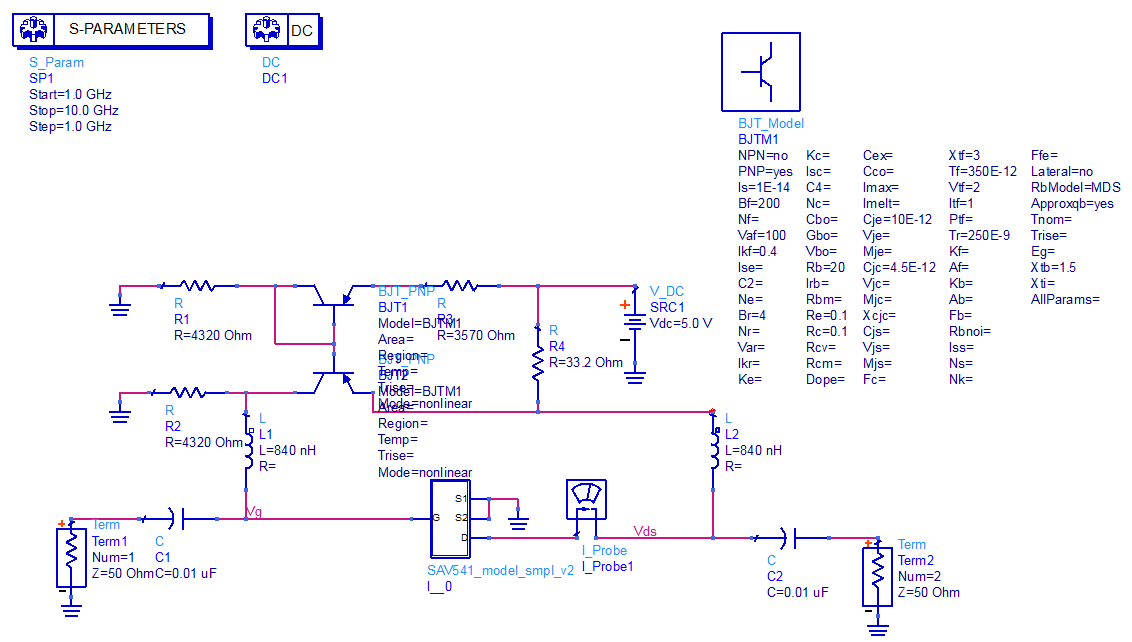
\includegraphics[width=2.5in]{pics/DCBiasNetwork.png}
\caption{DC bias network for the SAV-541+ transistor.}
\label{fig:dccircuit}
\end{figure}

\begin{figure}[!h]
\centering
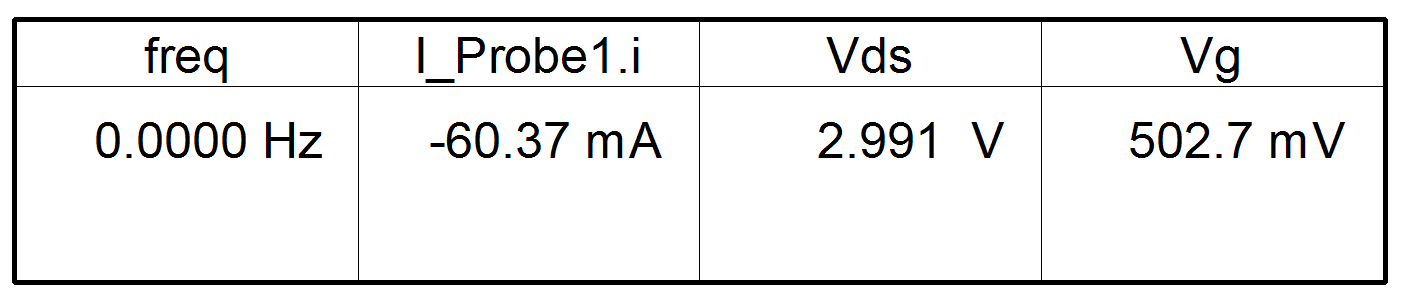
\includegraphics[width=2.5in]{pics/DCBiasResults.png}
\caption{Current and voltage parameters from the DC bias network for the SAV-541+ transistor.}
\label{fig:dcvalues}
\end{figure}

\begin{figure}[!h]
\centering
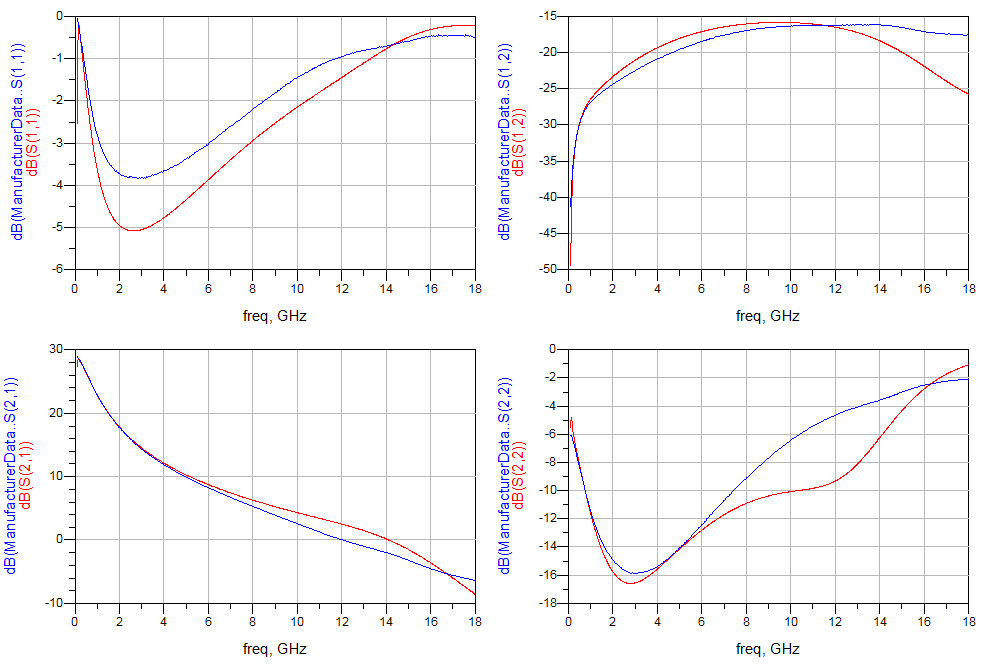
\includegraphics[width=2.5in]{pics/SParameterComparison.png}
\caption{S-Parameter simulation result comparison between the bias network and the manufacturer S2P data file.}
\label{fig:sparamresult}
\end{figure}

Figure~\ref{fig:designguide} shows various information provided by the ADS amplifier design guide tool. Observing the Stability Factor, K ($mu_{source}$/$mu_{load}$) graph, the circuit is potentially unstable below around 4 GHz. Thus, stabilizing resistors will be necessary in order to make the transistor unconditionally stable between 2.4 - 2.6 GHz (the intended frequency range).

\begin{figure}[!h]
\centering
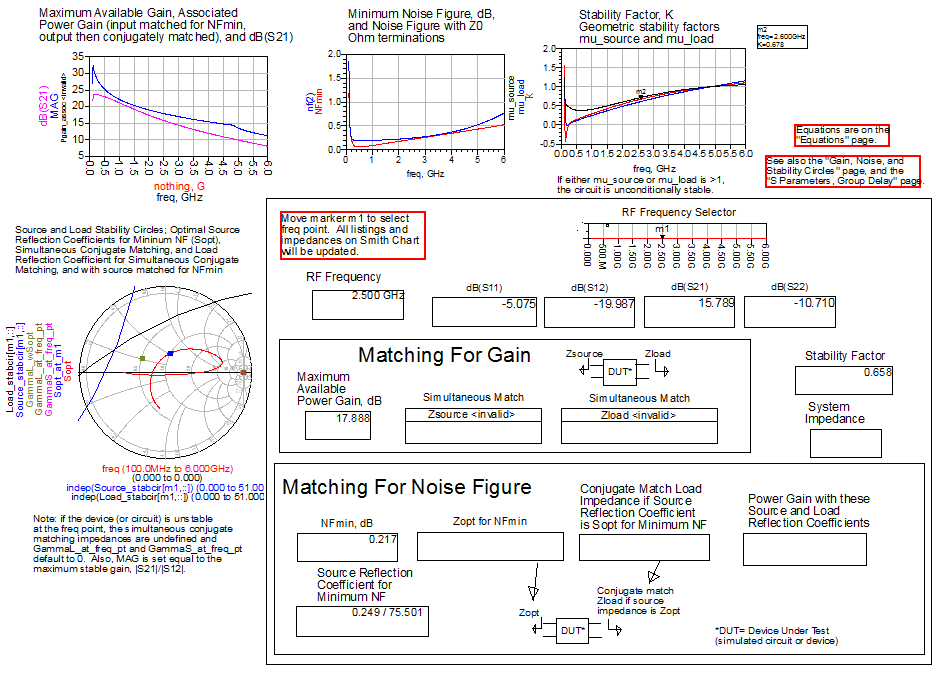
\includegraphics[width=2.5in]{pics/DesignGuideUnoptimized.png}
\caption{Amplifier design guide generated in ADS for the bias network for the SAV-541+ transistor.}
\label{fig:designguide}
\end{figure}

Figure~\ref{fig:designcuidecircuitstabilized} shows added feedback to the transistor used to stabilize it unconditionally (under 3 GHz). After tweaking the circuit for stability, Figure~\ref{fig:designcuidesimulationstabilized} shows the Design Guide for the stabilized circuit. It shows the circuit is unconditionally stable with a gain of 12.225 dB.

\begin{figure}[!h]
\centering
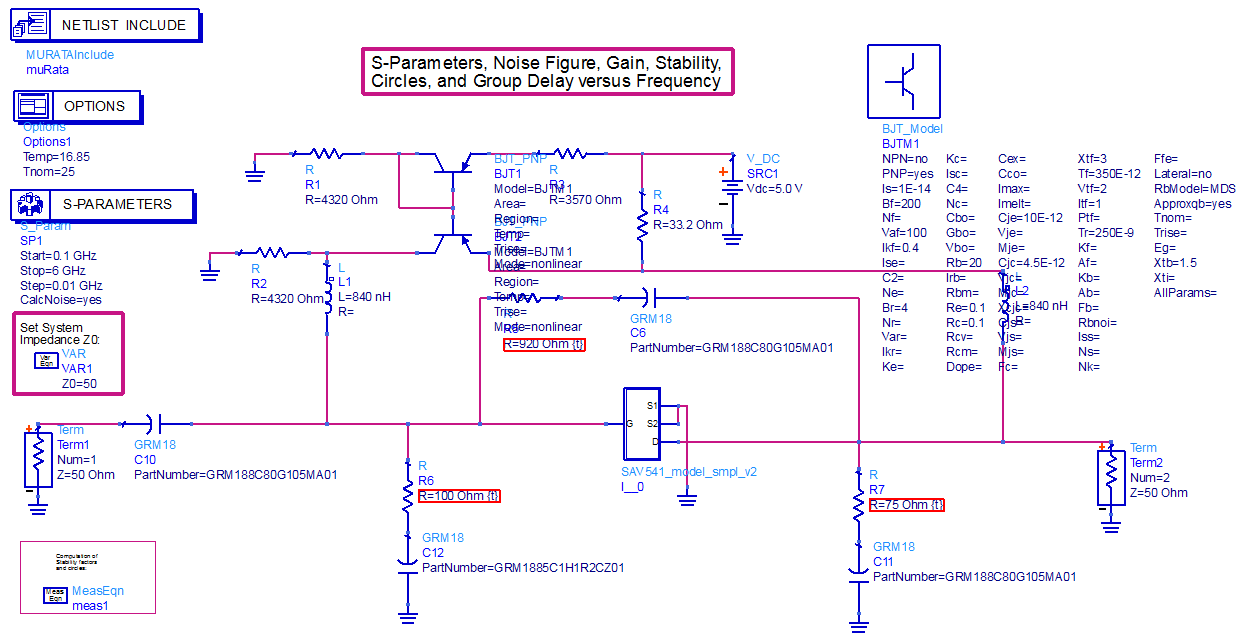
\includegraphics[width=2.5in]{pics/DesignGuideStablizedCircuit.png}
\caption{Stabilized transistor bias circuit for the SAV-541+ using feedback and stabilizing resistors.}
\label{fig:designcuidecircuitstabilized}
\end{figure}

\begin{figure}[!h]
\centering
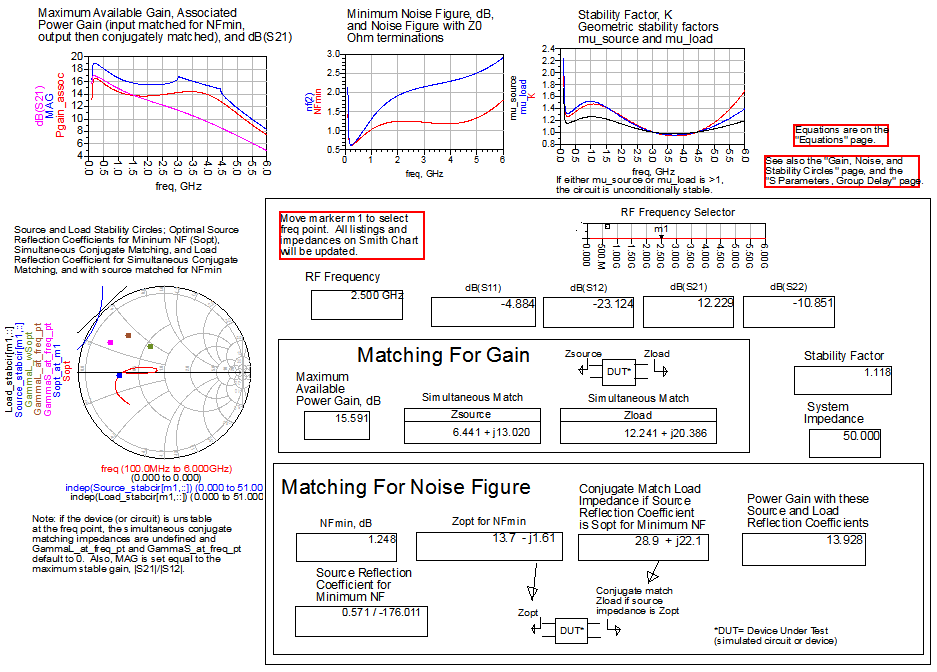
\includegraphics[width=2.5in]{pics/DesignGuideStablizedSimulation.png}
\caption{Amplifier design guide generated in ADS for the bias network for the SAV-541+ transistor.}
\label{fig:designcuidesimulationstabilized}
\end{figure}

Following ideal modeling, transmission lines were added to replace the ideal wires. As expected, adding transmission lines to the circuit caused the transistor to become potentially unstable. Thus, it was required to tune the feedback components again. Figure~\ref{fig:finalstabcircuit} shows the finalized stabilizing circuit for the SAV-541+ transistor. Figure~\ref{fig:finalstabsimulation} shows the design guide plots and shows the gain is above 10 dB.

Figure~\ref{fig:lnaLayout} shows the layout which will be used to manufacture the physical board.  This circuit was mechanically routed on what was assumed to be FR4, this was however not the case. After assembly, the LNA was analyzed using a PNA and found not produce any gain. The circuit was then powered with a bench supply and it was noticed that the current draw of the biasing network varied significantly with time. Further analysis was conducted using the PNA and it was determined that the amplifier was oscillating at various frequencies. The matching network and feedback network were checked to ensure that the proper values had been used. No errors were found. Despite our best efforts this design was never observed to provide stable gain.

Due to the extended period of time that was spent working on the LNA, several other labs were significantly delayed. The amount of work piling up for the FSK project lead to abandoning the LNA's development. A MMIC Amplifier was used instead to good effect. 

\begin{figure}[!h]
\centering
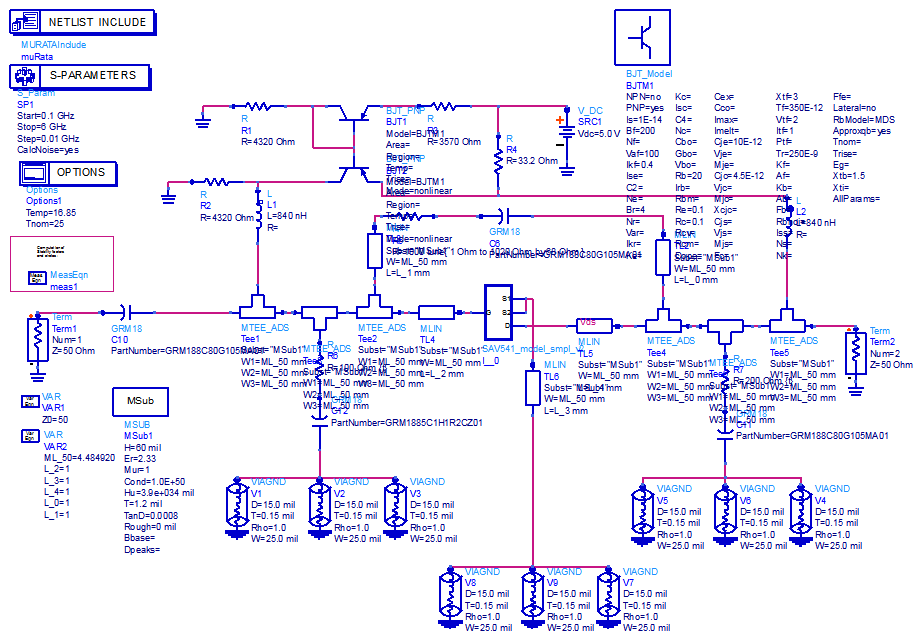
\includegraphics[width=2.5in]{pics/FinalStabilizingCircuit.png}
\caption{Final stabilizing circuit for the SAV-541+ transistor.}
\label{fig:finalstabcircuit}
\end{figure}

\begin{figure}[!h]
\centering
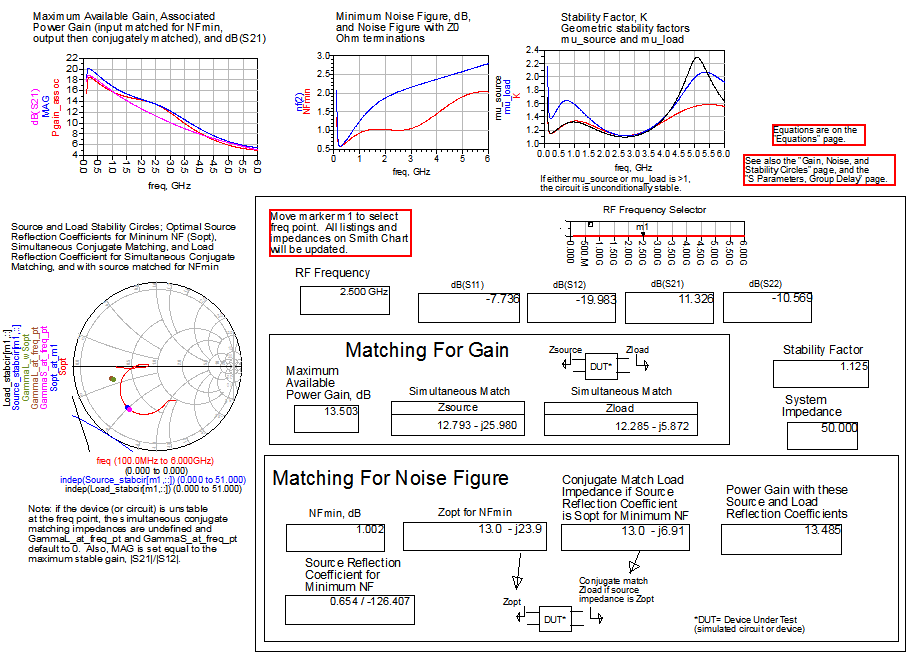
\includegraphics[width=2.5in]{pics/FinalStabilizingSimulation.png}
\caption{ADS design guide simulation results for the stabilizing circuit for the SAV-541+ transistor.}
\label{fig:finalstabsimulation}
\end{figure}

\begin{figure}[!h]
\centering
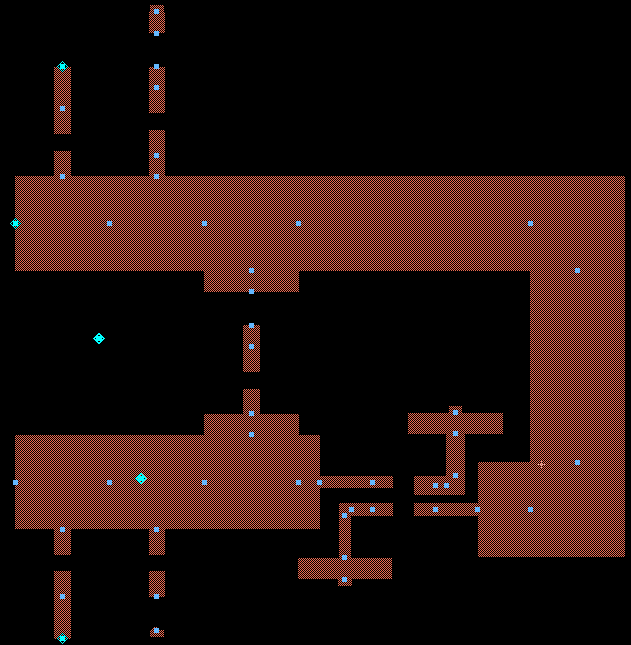
\includegraphics[width=2.5in]{LNApics/LNAlayout.png}
\caption{SAV-541+ transistor layout.}
\label{fig:lnaLayout}
\end{figure}

\section{Conclusion}
In summary, an LNA designed to the specifications given in Table~\ref{tab:specs} was designed, simulated, and built. The design and simulation of the LNA were consistent with expectations. The assembled LNA was inconsistent with both the simulations and the designer's expectations. The root cause of this inconsistency was not isolated despite attempts to do so. The authors' working assumption is that the substrate used had a significant variation from typical FR4 in terms of $E_r$ and that it was this variation that caused the instability. Other possibilities include mismarked components or damaged components. 

Lessons learned during this project included the importance of properly selecting and verifying all circuit elements used at microwave frequencies and the importance of physical testing as a means to augment computational modeling. While the authors' currently theorize that the oscillations were caused by variations in the circuit elements used in assembly, it is also possible that the issue was due to ADS's simulation providing erroneous results. Thus by testing a physical prototype, the designer can be assured that the models used accurately predict the behavior of the circuit designed.

Despite the eventual failure of the LNA designed for this project, the authors are confident that if presented with another LNA design task that a stable LNA could be implemented to reasonable specifications. This project provided valuable insight into the simulation process and how ADS works. Additional insight was gained into the process of prototyping microwave circuits with a mechanical circuit router.
\begin{thebibliography}{1}
\bibitem{sav541datasheet}
Minicircuit SAV-541+ Datasheet
\end{thebibliography}
\end{document}
